\documentclass[aspectratio=169]{beamer}

% -------------------------
% Basic packages
% -------------------------
\usepackage[utf8]{inputenc}
\usepackage{graphicx}
\usepackage{amsmath, amssymb}
\usepackage{booktabs}
\usepackage{array}
\usepackage{tikz}
\usepackage{tcolorbox}
\usepackage{hyperref}
\definecolor{questionbg}{RGB}{235, 244, 255}
\definecolor{questionframe}{RGB}{44, 95, 173}
\definecolor{plainbg}{RGB}{241, 249, 241}
\definecolor{plainframe}{RGB}{44, 122, 70}
\definecolor{notationbg}{RGB}{255, 248, 230}
\definecolor{notationframe}{RGB}{176, 118, 0}

\newtcolorbox{questionbox}{
  colback=questionbg,
  colframe=questionframe,
  boxrule=0.7pt,
  arc=1mm,
  fontupper=\small,
  left=1mm,
  right=1mm,
  top=0.4mm,
  bottom=0.4mm
}

\newtcolorbox{plainbox}{
  colback=plainbg,
  colframe=plainframe,
  boxrule=0.7pt,
  arc=1mm,
  fontupper=\small,
  left=1mm,
  right=1mm,
  top=0.4mm,
  bottom=0.4mm
}

\newtcolorbox{notationbox}{
  colback=notationbg,
  colframe=notationframe,
  boxrule=0.7pt,
  arc=1mm,
  fontupper=\small,
  left=1mm,
  right=1mm,
  top=0.4mm,
  bottom=0.4mm
}

\newcommand{\keyquestion}[1]{%
  \begin{questionbox}
  \textbf{Question:} #1
  \end{questionbox}
}

\newcommand{\plainidea}[1]{%
  \begin{plainbox}
  \textbf{Main idea:} #1
  \end{plainbox}
}

\newcommand{\notationblock}[1]{%
  \begin{notationbox}
  \textbf{Symbols used on this slide}\\
  #1
  \end{notationbox}
}

\newcommand{\exercisebreakcontent}[1]{%
  \begin{center}
  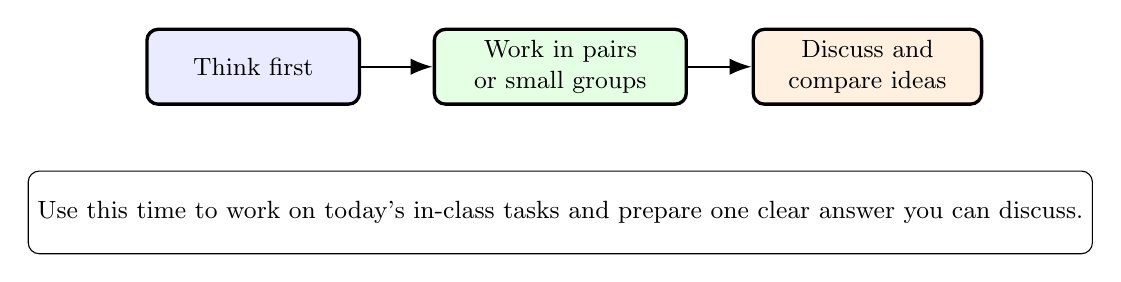
\begin{tikzpicture}[>=Latex, every node/.style={font=\small}]
    \node[draw, rounded corners, very thick, fill=blue!8, minimum width=2.7cm, minimum height=0.95cm, align=center] (think) at (-3.9,0.9) {Think first};
    \node[draw, rounded corners, very thick, fill=green!10, minimum width=3.2cm, minimum height=0.95cm, align=center] (work) at (0,0.9) {Work in pairs\\or small groups};
    \node[draw, rounded corners, very thick, fill=orange!12, minimum width=2.9cm, minimum height=0.95cm, align=center] (share) at (3.9,0.9) {Discuss and\\compare ideas};
    \draw[-{Latex[length=2.8mm]}, thick] (think) -- (work);
    \draw[-{Latex[length=2.8mm]}, thick] (work) -- (share);
    \node[draw, rounded corners, fill=white, minimum width=9.4cm, minimum height=1.05cm, align=center] at (0,-0.95) {Use this time to work on today's in-class tasks and prepare one clear answer you can discuss.};
  \end{tikzpicture}
  \end{center}
  \plainidea{#1}
}

\usetikzlibrary{positioning,arrows.meta,fit}

% -------------------------
% Theme
% -------------------------
\usetheme{Madrid}
\usecolortheme{default}
\setbeamertemplate{navigation symbols}{}

% -------------------------
% Per-slide reference footer
% -------------------------
\newcommand{\defaultdeckrefs}{AIMA4e Ch.12--13 pp.385--460; Poole3e Ch.9 pp.375--458}
\newcommand{\currentsliderefs}{\defaultdeckrefs}
\newcommand{\setslideref}[1]{\gdef\currentsliderefs{#1}}
\addtobeamertemplate{footline}{}{%
  \begin{beamercolorbox}[wd=\paperwidth,leftskip=0.4em,rightskip=0.4em,ht=2.8ex,dp=0.9ex]{author in head/foot}
    \tiny\textbf{Refs: }\currentsliderefs
  \end{beamercolorbox}
}

% -------------------------
% Metadata
% -------------------------
\title[EBU6505 B4 D1]{EBU6505 -- Reasoning and Agents\\Block 4, Day 1 -- Bayesian Networks}
\author{Dr Riasat Islam}
\institute{Queen Mary University of London}
\date{}

% -------------------------
% TikZ styles
% -------------------------
\tikzset{
  flowarrow/.style={-{Latex[length=2.8mm]}, thick},
  bnnode/.style={draw, rounded corners, very thick, fill=blue!8, minimum width=2.3cm, minimum height=0.95cm, align=center},
  obsnode/.style={draw, rounded corners, very thick, fill=green!10, minimum width=2.3cm, minimum height=0.95cm, align=center},
  note/.style={draw, rounded corners, fill=orange!12, minimum width=2.4cm, minimum height=0.95cm, align=center},
  softbox/.style={draw, rounded corners, fill=white, minimum width=2.6cm, minimum height=0.95cm, align=center},
  relabel/.style={font=\small, fill=white, inner sep=1pt}
}

\begin{document}

\setslideref{AIMA4e Ch.12--13 pp.385--460; Poole3e Ch.9 pp.375--458}
\begin{frame}
  \titlepage
\end{frame}

\begin{frame}{What have we covered so far this module?}
\begin{itemize}
  \item reasoning techniques for LLMs and test-time compute
  \item search and state-space problem solving
  \item MDPs and reinforcement learning
  \item knowledge representation and knowledge graphs
  \item graph-based reasoning for retrieval, memory, and agents
\end{itemize}
\plainidea{Block 4 starts a new question: what should an agent believe when the world is uncertain and the evidence is incomplete?}
\end{frame}

\begin{frame}{What are we going to cover this week?}
\begin{itemize}
  \item Day 1: Bayesian networks
  \item Day 2: exact inference in Bayesian networks
  \item Day 3: probabilistic reasoning over time
  \item Day 4: planning with uncertainty
  \item Day 5: decision networks and POMDP synthesis
\end{itemize}
\plainidea{This week moves from structured knowledge to uncertain knowledge: first model it, then infer with it, then plan with it.}
\end{frame}

\begin{frame}{What are we going to cover today?}
\begin{itemize}
  \item why Bayesian networks are useful for uncertain reasoning
  \item what nodes, arrows, and CPTs mean
  \item how a network represents a full joint distribution
  \item how conditional independence and d-separation work
  \item what kind of inference question we will solve next
\end{itemize}
\plainidea{Today is the foundation lecture. Students do not need heavy calculations yet; they need a clear mental model first.}
\end{frame}

\begin{frame}{Resources}
\small
\begin{itemize}
  \item \textit{Artificial Intelligence: Foundations of Computational Agents}, David Poole and Alan Mackworth (3rd ed.)
  \item Poole 3e, Chapter 9: Reasoning with Uncertainty
  \item \textit{Artificial Intelligence: A Modern Approach}, Russell and Norvig (4th ed.)
  \item AIMA 4e, Chapter 12: Quantifying Uncertainty
  \item AIMA 4e, Chapter 13: Probabilistic Reasoning
\end{itemize}
\plainidea{The two textbooks say the same core thing in different ways: a Bayesian network gives a graph structure plus probability tables.}
\end{frame}

\begin{frame}{Learning Outcomes for Today}
\begin{itemize}
  \item explain what a Bayesian network is in simple words
  \item read the meaning of nodes, arrows, and CPTs
  \item explain why the graph reduces the size of the probability model
  \item identify the three common d-separation patterns
  \item interpret a simple inference query with evidence
\end{itemize}
\plainidea{If students leave with these five ideas clear, Day 2 calculations become much easier.}
\end{frame}

\begin{frame}{Warm-Up Question}
\keyquestion{If a patient has a fever, can we be 100\% sure they have flu?}
\begin{columns}[T,onlytextwidth]
  \begin{column}{0.48\textwidth}
    \begin{tcolorbox}[colback=questionbg,colframe=questionframe,boxrule=0.7pt,title=What we know]
    Fever is evidence, not proof.
    \end{tcolorbox}
  \end{column}
  \begin{column}{0.48\textwidth}
    \begin{tcolorbox}[colback=plainbg,colframe=plainframe,boxrule=0.7pt,title=Why]
    Different causes can lead to the same symptom.
    \end{tcolorbox}
  \end{column}
\end{columns}
\begin{center}
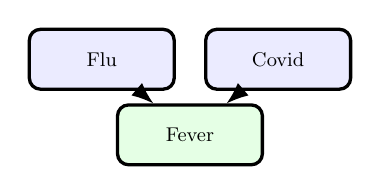
\begin{tikzpicture}[>=Latex, scale=0.8, every node/.style={font=\small, transform shape}]
  \node[bnnode] (flu) at (0,0.2) {Flu};
  \node[bnnode] (covid) at (2.8,0.2) {Covid};
  \node[obsnode] (fever) at (1.4,-1.0) {Fever};
  \draw[flowarrow] (flu) -- (fever);
  \draw[flowarrow] (covid) -- (fever);
\end{tikzpicture}
\end{center}
\vspace{-0.35em}
\plainidea{Uncertain symptoms need probabilistic reasoning, not yes-or-no rules.}
\end{frame}

\begin{frame}{What Problem Does a Bayesian Network Solve?}
\keyquestion{Why not just write one huge probability table for every variable together?}
\begin{columns}[T,onlytextwidth]
  \begin{column}{0.48\textwidth}
    \begin{tcolorbox}[colback=questionbg,colframe=questionframe,boxrule=0.7pt,title=One huge table]
    Hard to read, hard to estimate, and grows fast as we add variables.
    \end{tcolorbox}
  \end{column}
  \begin{column}{0.48\textwidth}
    \begin{tcolorbox}[colback=plainbg,colframe=plainframe,boxrule=0.7pt,title=Bayesian network]
    Split the model into small local pieces connected by a graph.
    \end{tcolorbox}
  \end{column}
\end{columns}
\begin{center}
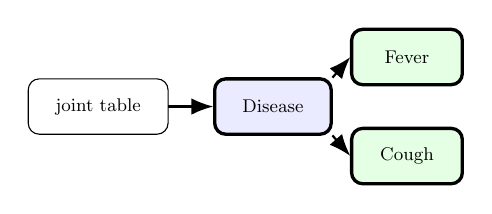
\begin{tikzpicture}[>=Latex, scale=0.74, every node/.style={font=\small, transform shape}]
  \node[softbox, minimum width=2.4cm] (joint) at (0,0.05) {joint table};
  \node[bnnode, minimum width=2.0cm] (disease) at (3.0,0.05) {Disease};
  \node[obsnode, minimum width=1.9cm] (fever) at (5.3,0.9) {Fever};
  \node[obsnode, minimum width=1.9cm] (cough) at (5.3,-0.8) {Cough};
  \draw[flowarrow] (joint.east) -- (disease.west);
  \draw[flowarrow] (disease.north east) -- (fever.west);
  \draw[flowarrow] (disease.south east) -- (cough.west);
\end{tikzpicture}
\end{center}
\vspace{-0.35em}
\plainidea{A BN replaces one huge table with small connected pieces.}
\end{frame}

\begin{frame}{What Is a Bayesian Network?}
\keyquestion{What are the two parts of a Bayesian network?}
\begin{columns}[T,onlytextwidth]
  \begin{column}{0.52\textwidth}
    \begin{itemize}
      \item a \textbf{graph} that shows which variables directly depend on which others
      \item a \textbf{CPT} for each node that gives the probability numbers
      \item the graph is directed, and it must not contain a cycle
    \end{itemize}
    \plainidea{A Bayesian network is a directed acyclic graph plus one local probability table for each variable.}
  \end{column}
  \begin{column}{0.48\textwidth}
    \begin{center}
    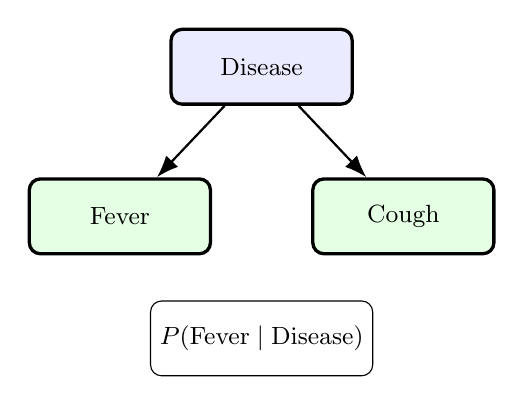
\begin{tikzpicture}[>=Latex, every node/.style={font=\small}]
      \node[bnnode] (d) at (0,1.0) {Disease};
      \node[obsnode] (f) at (-1.8,-0.9) {Fever};
      \node[obsnode] (c) at (1.8,-0.9) {Cough};
      \draw[flowarrow] (d) -- (f);
      \draw[flowarrow] (d) -- (c);
      \node[softbox, minimum width=2.7cm] at (0,-2.45) {$P(\text{Fever}\mid \text{Disease})$};
    \end{tikzpicture}
    \end{center}
  \end{column}
\end{columns}
\end{frame}

\begin{frame}{How Do We Read a Small Bayesian Network?}
\keyquestion{What does the graph say in simple words?}
\small
\begin{center}
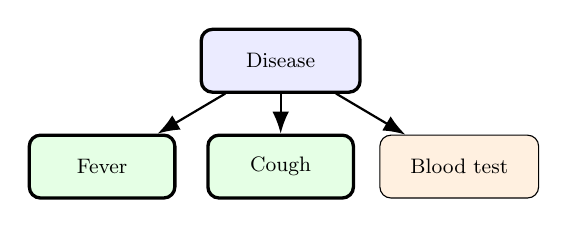
\begin{tikzpicture}[>=Latex, scale=0.84, every node/.style={font=\small, transform shape}]
  \node[bnnode, minimum width=2.4cm] (d) at (0,0.6) {Disease};
  \node[obsnode, minimum width=2.2cm] (f) at (-2.7,-1.0) {Fever};
  \node[obsnode, minimum width=2.2cm] (c) at (0,-1.0) {Cough};
  \node[note, minimum width=2.4cm] (t) at (2.7,-1.0) {Blood test};
  \draw[flowarrow] (d) -- (f);
  \draw[flowarrow] (d) -- (c);
  \draw[flowarrow] (d) -- (t);
\end{tikzpicture}
\end{center}
\begin{columns}[T,onlytextwidth]
  \begin{column}{0.32\textwidth}
    \begin{tcolorbox}[colback=questionbg,colframe=questionframe,boxrule=0.7pt,title=Node]
    one uncertain variable
    \end{tcolorbox}
  \end{column}
  \begin{column}{0.32\textwidth}
    \begin{tcolorbox}[colback=plainbg,colframe=plainframe,boxrule=0.7pt,title=Arrow]
    direct influence
    \end{tcolorbox}
  \end{column}
  \begin{column}{0.32\textwidth}
    \begin{tcolorbox}[colback=notationbg,colframe=notationframe,boxrule=0.7pt,title=CPT]
    local probabilities
    \end{tcolorbox}
  \end{column}
\end{columns}
\vspace{-0.35em}
\plainidea{This graph says Disease directly changes the probability of Fever, Cough, and the Test result.}
\end{frame}

\begin{frame}{Why Is the Graph Better Than One Giant Table?}
\keyquestion{What does the graph save us from writing down?}
\small
\begin{columns}[T,onlytextwidth]
  \begin{column}{0.48\textwidth}
    \begin{tcolorbox}[colback=questionbg,colframe=questionframe,boxrule=0.7pt,title=Without structure]
    \begin{itemize}
      \item one big joint table
      \item many combinations
      \item hard to explain
    \end{itemize}
    \end{tcolorbox}
  \end{column}
  \begin{column}{0.48\textwidth}
    \begin{tcolorbox}[colback=plainbg,colframe=plainframe,boxrule=0.7pt,title=With structure]
    \begin{itemize}
      \item one small table per node
      \item local dependencies only
      \item easier to read and update
    \end{itemize}
    \end{tcolorbox}
  \end{column}
\end{columns}
\vspace{-0.45em}
\begin{center}
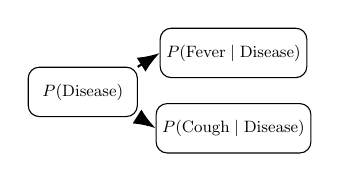
\begin{tikzpicture}[>=Latex, scale=0.66, every node/.style={font=\small, transform shape}]
  \node[softbox, minimum width=2.1cm] (p1) at (0,0.15) {$P(\text{Disease})$};
  \node[softbox, minimum width=2.4cm] (p2) at (2.9,0.9) {$P(\text{Fever}\mid \text{Disease})$};
  \node[softbox, minimum width=2.4cm] (p3) at (2.9,-0.55) {$P(\text{Cough}\mid \text{Disease})$};
  \draw[flowarrow] (p1.north east) -- (p2.west);
  \draw[flowarrow] (p1.south east) -- (p3.west);
\end{tikzpicture}
\end{center}
\vspace{-0.55em}
\plainidea{The graph tells us which local tables we need.}
\end{frame}

\begin{frame}{Where Do CPT Numbers Come From?}
\keyquestion{How do we fill in the probabilities on the nodes?}
\begin{columns}[T,onlytextwidth]
  \begin{column}{0.31\textwidth}
    \begin{tcolorbox}[colback=questionbg,colframe=questionframe,boxrule=0.7pt,title=Experts]
    doctors, engineers, or domain specialists estimate the numbers
    \end{tcolorbox}
  \end{column}
  \begin{column}{0.31\textwidth}
    \begin{tcolorbox}[colback=plainbg,colframe=plainframe,boxrule=0.7pt,title=Data]
    count frequencies from records
    \end{tcolorbox}
  \end{column}
  \begin{column}{0.31\textwidth}
    \begin{tcolorbox}[colback=notationbg,colframe=notationframe,boxrule=0.7pt,title=Toy models]
    use temporary values for teaching or early design
    \end{tcolorbox}
  \end{column}
\end{columns}
\plainidea{CPTs are not magic. They come from people, data, or temporary assumptions used for teaching and early design.}
\end{frame}

\begin{frame}{Example CPT: Fever Given Disease}
\keyquestion{How do we read one local probability table?}
\begin{columns}[T,onlytextwidth]
  \begin{column}{0.46\textwidth}
    \begin{center}
    \begin{tabular}{lcc}
    \toprule
    Disease & $P(Fever=T)$ & $P(Fever=F)$ \\
    \midrule
    Flu & 0.8 & 0.2 \\
    No flu & 0.2 & 0.8 \\
    \bottomrule
    \end{tabular}
    \end{center}
  \end{column}
  \begin{column}{0.50\textwidth}
    \begin{tcolorbox}[colback=plainbg,colframe=plainframe,boxrule=0.7pt,title=How to read it]
    If the patient has flu, the model gives a high probability of fever.
    If the patient does not have flu, fever is still possible, but less likely.
    \end{tcolorbox}
  \end{column}
\end{columns}
\plainidea{A CPT is always local: one node, its parents, and the probabilities for that small situation only.}
\end{frame}

\begin{frame}{How Does the Whole Network Define One Probability Model?}
\keyquestion{How do the local tables combine into one joint distribution?}
\begin{center}
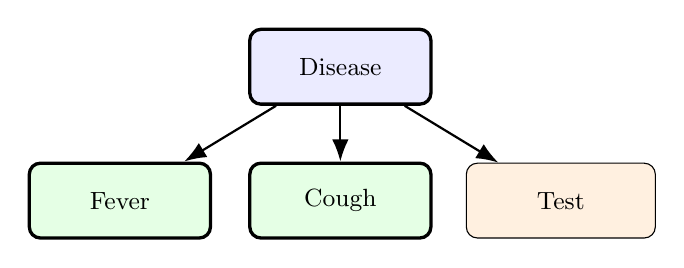
\begin{tikzpicture}[>=Latex, every node/.style={font=\small}]
  \node[bnnode] (d) at (0,0.7) {Disease};
  \node[obsnode] (f) at (-2.8,-1.0) {Fever};
  \node[obsnode] (c) at (0,-1.0) {Cough};
  \node[note] (t) at (2.8,-1.0) {Test};
  \draw[flowarrow] (d) -- (f);
  \draw[flowarrow] (d) -- (c);
  \draw[flowarrow] (d) -- (t);
\end{tikzpicture}
\end{center}
\[
P(D,F,C,T)=P(D)\,P(F\mid D)\,P(C\mid D)\,P(T\mid D)
\]
\plainidea{The graph tells us how to break one large joint probability into smaller local factors.}
\end{frame}

\begin{frame}{What Does Conditional Independence Mean Here?}
\keyquestion{When does one symptom stop giving extra information about another?}
\begin{center}
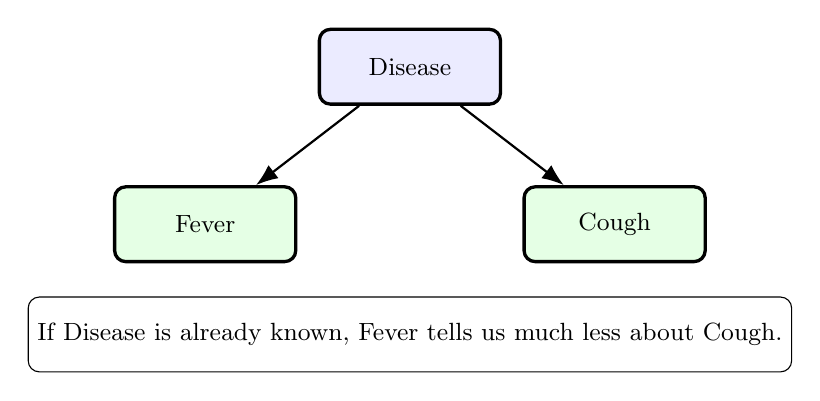
\begin{tikzpicture}[>=Latex, every node/.style={font=\small}]
  \node[bnnode] (d) at (0,1.0) {Disease};
  \node[obsnode] (f) at (-2.6,-1.0) {Fever};
  \node[obsnode] (c) at (2.6,-1.0) {Cough};
  \draw[flowarrow] (d) -- (f);
  \draw[flowarrow] (d) -- (c);
  \node[softbox, minimum width=4.7cm] at (0,-2.4) {If Disease is already known, Fever tells us much less about Cough.};
\end{tikzpicture}
\end{center}
\plainidea{Conditional independence means some variables stop sharing extra information once we already know the right middle variable.}
\end{frame}

\begin{frame}{What Is D-Separation?}
\keyquestion{How can we decide from the graph whether information can still flow along a path?}
\begin{columns}[T,onlytextwidth]
  \begin{column}{0.52\textwidth}
    \begin{itemize}
      \item pick a path between two variables
      \item look at the middle node pattern
      \item ask whether that middle node is observed
      \item decide whether the path is open or blocked
    \end{itemize}
  \end{column}
  \begin{column}{0.44\textwidth}
    \begin{center}
    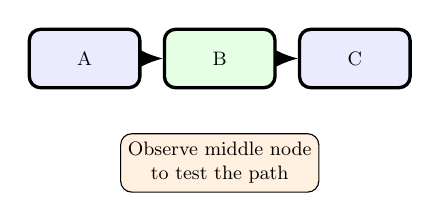
\begin{tikzpicture}[>=Latex, scale=0.78, every node/.style={font=\small, transform shape}]
      \node[bnnode, minimum width=1.8cm] (a) at (0,0) {A};
      \node[obsnode, minimum width=1.8cm] (b) at (2.2,0) {B};
      \node[bnnode, minimum width=1.8cm] (c) at (4.4,0) {C};
      \draw[flowarrow] (a.east) -- (b.west);
      \draw[flowarrow] (b.east) -- (c.west);
      \node[note, minimum width=2.4cm] at (2.2,-1.7) {Observe middle node\\to test the path};
    \end{tikzpicture}
    \end{center}
  \end{column}
\end{columns}
\plainidea{Students can think of d-separation as an information-flow test: does evidence travel through this path or does the path stop it?}
\end{frame}

\begin{frame}{Three Common D-Separation Patterns}
\keyquestion{Which middle-node pattern are we looking at?}
\small
\begin{columns}[T,onlytextwidth]
  \begin{column}{0.32\textwidth}
    \begin{center}
    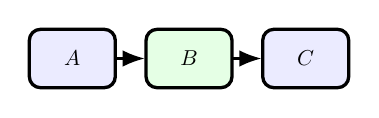
\begin{tikzpicture}[>=Latex, scale=0.78, every node/.style={transform shape}]
      \node[bnnode, minimum width=1.4cm] (a1) at (0,0) {$A$};
      \node[obsnode, minimum width=1.4cm] (b1) at (1.9,0) {$B$};
      \node[bnnode, minimum width=1.4cm] (c1) at (3.8,0) {$C$};
      \draw[flowarrow] (a1) -- (b1);
      \draw[flowarrow] (b1) -- (c1);
    \end{tikzpicture}

    \textbf{Serial chain}\\
    observe $B$ to block
    \end{center}
  \end{column}
  \begin{column}{0.32\textwidth}
    \begin{center}
    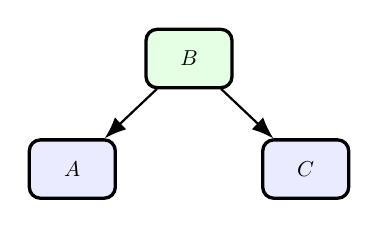
\begin{tikzpicture}[>=Latex, scale=0.78, every node/.style={transform shape}]
      \node[obsnode, minimum width=1.4cm] (b2) at (1.9,0.9) {$B$};
      \node[bnnode, minimum width=1.4cm] (a2) at (0,-0.9) {$A$};
      \node[bnnode, minimum width=1.4cm] (c2) at (3.8,-0.9) {$C$};
      \draw[flowarrow] (b2) -- (a2);
      \draw[flowarrow] (b2) -- (c2);
    \end{tikzpicture}

    \textbf{Common cause}\\
    observe $B$ to block
    \end{center}
  \end{column}
  \begin{column}{0.32\textwidth}
    \begin{center}
    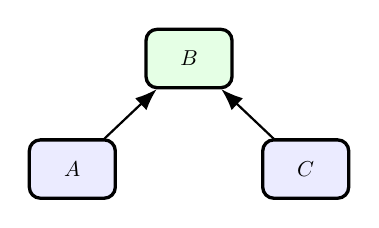
\begin{tikzpicture}[>=Latex, scale=0.78, every node/.style={transform shape}]
      \node[bnnode, minimum width=1.4cm] (a3) at (0,-0.9) {$A$};
      \node[obsnode, minimum width=1.4cm] (b3) at (1.9,0.9) {$B$};
      \node[bnnode, minimum width=1.4cm] (c3) at (3.8,-0.9) {$C$};
      \draw[flowarrow] (a3) -- (b3);
      \draw[flowarrow] (c3) -- (b3);
    \end{tikzpicture}

    \textbf{Collider}\\
    observe $B$ to open
    \end{center}
  \end{column}
\end{columns}
\plainidea{The collider case is the unusual one. It behaves in the opposite way from the first two patterns.}
\end{frame}

\begin{frame}{Pattern 1: Serial Chain}
\keyquestion{What happens in a chain when we observe the middle variable?}
\begin{columns}[T,onlytextwidth]
  \begin{column}{0.58\textwidth}
    \begin{itemize}
      \item structure: $A \rightarrow B \rightarrow C$
      \item before we know $B$, information can travel from $A$ to $C$
      \item after we know $B$, the path is blocked
    \end{itemize}
    \begin{tcolorbox}[colback=plainbg,colframe=plainframe,boxrule=0.7pt,title=Example]
    Rain $\rightarrow$ Wet road $\rightarrow$ Traffic delay
    \end{tcolorbox}
  \end{column}
  \begin{column}{0.38\textwidth}
    \begin{center}
    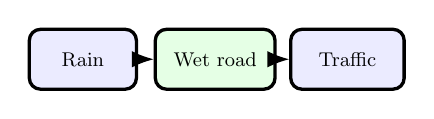
\begin{tikzpicture}[>=Latex, scale=0.8, every node/.style={font=\small, transform shape}]
      \node[bnnode, minimum width=1.7cm] (a) at (0,0) {Rain};
      \node[obsnode, minimum width=1.9cm] (b) at (2.1,0) {Wet road};
      \node[bnnode, minimum width=1.8cm] (c) at (4.2,0) {Traffic};
      \draw[flowarrow] (a) -- (b);
      \draw[flowarrow] (b) -- (c);
    \end{tikzpicture}
    \end{center}
  \end{column}
\end{columns}
\plainidea{In a serial chain, observing the middle node blocks the path.}
\end{frame}

\begin{frame}{Pattern 2: Common Cause}
\keyquestion{What happens when two effects share the same cause?}
\begin{columns}[T,onlytextwidth]
  \begin{column}{0.58\textwidth}
    \begin{itemize}
      \item structure: $A \leftarrow B \rightarrow C$
      \item before we know $B$, the two effects can look related
      \item after we know $B$, that path is blocked
    \end{itemize}
    \begin{tcolorbox}[colback=plainbg,colframe=plainframe,boxrule=0.7pt,title=Example]
    Fever $\leftarrow$ Disease $\rightarrow$ Cough
    \end{tcolorbox}
  \end{column}
  \begin{column}{0.38\textwidth}
    \begin{center}
    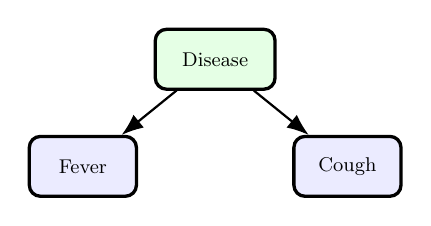
\begin{tikzpicture}[>=Latex, scale=0.8, every node/.style={font=\small, transform shape}]
      \node[obsnode, minimum width=1.9cm] (b) at (2.1,0.8) {Disease};
      \node[bnnode, minimum width=1.7cm] (a) at (0,-0.9) {Fever};
      \node[bnnode, minimum width=1.7cm] (c) at (4.2,-0.9) {Cough};
      \draw[flowarrow] (b) -- (a);
      \draw[flowarrow] (b) -- (c);
    \end{tikzpicture}
    \end{center}
  \end{column}
\end{columns}
\plainidea{In a common-cause pattern, observing the shared cause blocks the path between the effects.}
\end{frame}

\begin{frame}{Pattern 3: Collider}
\keyquestion{Why is the collider pattern different from the first two?}
\begin{columns}[T,onlytextwidth]
  \begin{column}{0.58\textwidth}
    \begin{itemize}
      \item structure: $A \rightarrow B \leftarrow C$
      \item before we know $B$, the path is blocked
      \item after we know $B$ or its descendant, the path opens
    \end{itemize}
    \begin{tcolorbox}[colback=plainbg,colframe=plainframe,boxrule=0.7pt,title=Example]
    Burglary $\rightarrow$ Alarm $\leftarrow$ Earthquake
    \end{tcolorbox}
  \end{column}
  \begin{column}{0.38\textwidth}
    \begin{center}
    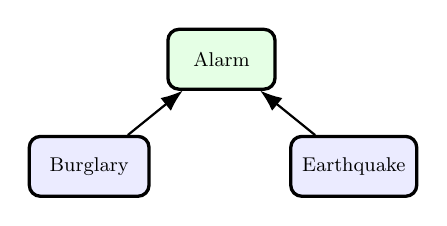
\begin{tikzpicture}[>=Latex, scale=0.8, every node/.style={font=\small, transform shape}]
      \node[bnnode, minimum width=1.9cm] (a) at (0,-0.9) {Burglary};
      \node[obsnode, minimum width=1.7cm] (b) at (2.1,0.8) {Alarm};
      \node[bnnode, minimum width=2.0cm] (c) at (4.2,-0.9) {Earthquake};
      \draw[flowarrow] (a) -- (b);
      \draw[flowarrow] (c) -- (b);
    \end{tikzpicture}
    \end{center}
  \end{column}
\end{columns}
\plainidea{In a collider, the path is closed by default. Observing the middle effect opens it.}
\end{frame}

\begin{frame}{What Is Inference in a Bayesian Network?}
\keyquestion{Once we have the network, what question do we usually ask?}
\begin{columns}[T,onlytextwidth]
  \begin{column}{0.48\textwidth}
    \begin{tcolorbox}[colback=questionbg,colframe=questionframe,boxrule=0.7pt,title=Evidence we observe]
    Fever = true\\
    Cough = true
    \end{tcolorbox}
    \begin{tcolorbox}[colback=plainbg,colframe=plainframe,boxrule=0.7pt,title=Hidden variable we ask about]
    What is the probability of Disease?
    \end{tcolorbox}
  \end{column}
  \begin{column}{0.48\textwidth}
    \[
    P(\text{Disease}\mid \text{Fever}=T,\text{Cough}=T)
    \]
    \begin{tcolorbox}[colback=notationbg,colframe=notationframe,boxrule=0.7pt]
    Read this as: probability of Disease given the evidence.
    \end{tcolorbox}
  \end{column}
\end{columns}
\plainidea{Inference means updating belief about an unknown variable after we observe evidence.}
\end{frame}

\begin{frame}{Where Are Bayesian Networks Useful?}
\keyquestion{What kinds of real tasks match this model well?}
\small
\begin{columns}[T,onlytextwidth]
  \begin{column}{0.31\textwidth}
    \begin{tcolorbox}[colback=questionbg,colframe=questionframe,boxrule=0.7pt,title=Healthcare]
    symptoms, tests,\\ diseases
    \end{tcolorbox}
  \end{column}
  \begin{column}{0.31\textwidth}
    \begin{tcolorbox}[colback=plainbg,colframe=plainframe,boxrule=0.7pt,title=Systems]
    faults, alarms,\\ missing sensors
    \end{tcolorbox}
  \end{column}
  \begin{column}{0.31\textwidth}
    \begin{tcolorbox}[colback=notationbg,colframe=notationframe,boxrule=0.7pt,title=Finance]
    market signals,\\ fraud clues, loss risk
    \end{tcolorbox}
  \end{column}
\end{columns}
\begin{center}
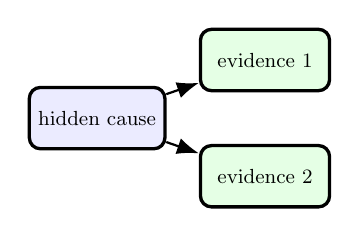
\begin{tikzpicture}[>=Latex, scale=0.82, every node/.style={font=\small, transform shape}]
  \node[bnnode, minimum width=2.1cm] (cause) at (0,0) {hidden cause};
  \node[obsnode, minimum width=2.0cm] (e1) at (2.6,0.9) {evidence 1};
  \node[obsnode, minimum width=2.0cm] (e2) at (2.6,-0.9) {evidence 2};
  \draw[flowarrow] (cause) -- (e1);
  \draw[flowarrow] (cause) -- (e2);
\end{tikzpicture}
\end{center}
\vspace{-0.35em}
\plainidea{Bayesian networks help when the real cause is hidden but we can observe uncertain clues.}
\end{frame}

\begin{frame}{How Does Day 1 Connect to Day 2?}
\keyquestion{What are we doing after we understand the model structure?}
\begin{center}
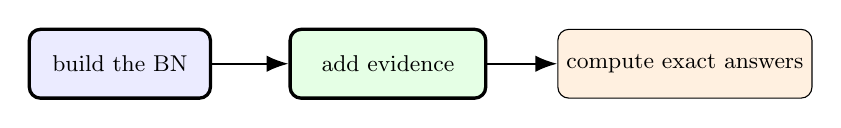
\begin{tikzpicture}[>=Latex, scale=0.92, every node/.style={font=\small, transform shape}]
  \node[bnnode, minimum width=2.5cm] (model) at (0,0) {build the BN};
  \node[obsnode, minimum width=2.7cm] (query) at (3.7,0) {add evidence};
  \node[note, minimum width=3.0cm] (infer) at (7.8,0) {compute exact answers};
  \draw[flowarrow] (model.east) -- (query.west);
  \draw[flowarrow] (query.east) -- (infer.west);
\end{tikzpicture}
\end{center}
\plainidea{Day 1 is about building and reading the model. Day 2 is about computing answers from that model.}
\end{frame}

\begin{frame}{Key Takeaways}
\begin{itemize}
  \item A Bayesian network is a directed acyclic graph plus one CPT per node.
  \item The graph makes a large uncertain model smaller and easier to explain.
  \item Conditional independence is one of the main reasons the model stays compact.
  \item D-separation is the graph test for deciding whether a path is open or blocked.
  \item Inference asks for the probability of something unknown given the evidence we observe.
\end{itemize}
\plainidea{The main lesson from Day 1 is simple: Bayesian networks separate structure from numbers, and that makes uncertain reasoning much easier to organise.}
\end{frame}

\begin{frame}{In-Class Exercises}
\exercisebreakcontent{Use the exercise time to move from the picture of a Bayesian network to the meaning of the variables, edges, and query.}
\end{frame}

\begin{frame}{Further Study}
\begin{itemize}
  \item Read Poole Chapter 9 and AIMA Chapters 12--13.
  \item Practice: Poole Ch.9, Exercises 9.2, 9.3, 9.4, and 9.7.
  \item AIMA Bayesian-network exercise page: 14.1, 14.5, 14.6, and 14.8.
  \item Focus on building the graph, reading conditional dependence, and explaining what changes when evidence is observed.
\end{itemize}
\end{frame}

\end{document}
